\documentclass{article}

% --- Encoding & Language ---
\usepackage[utf8]{inputenc}
\usepackage[british]{babel}
\usepackage{textgreek}
\DeclareUnicodeCharacter{2212}{\ensuremath{-}}
\DeclareUnicodeCharacter{2032}{\ensuremath{\prime}}
\DeclareUnicodeCharacter{2033}{\ensuremath{\prime\prime}}
\DeclareUnicodeCharacter{2080}{\ensuremath{_0}}
\DeclareUnicodeCharacter{2081}{\ensuremath{_1}}
\DeclareUnicodeCharacter{2084}{\ensuremath{_4}}
\DeclareUnicodeCharacter{2075}{\ensuremath{^5}}
\DeclareUnicodeCharacter{207B}{\ensuremath{^-}}

% --- Authors ---
\usepackage{authblk}
\usepackage{orcidlink}

% --- Page Layout ---
\usepackage[margin=1in, headsep=0.25in]{geometry}
\usepackage{setspace}
\usepackage{lineno}

% --- Graphics & Floats ---
\usepackage{graphicx}
\graphicspath{{./figures/}}
\usepackage{subcaption}
\usepackage{caption}
\usepackage{rotating}
\usepackage{float}
\renewcommand{\floatpagefraction}{0.1}

% --- Tables ---
\usepackage{booktabs}
\usepackage{multirow}
\usepackage{tabularx}
\usepackage{array}

% --- Math & Units ---
\usepackage{amsmath}
\usepackage{siunitx}

% --- Colors & Frames ---
\usepackage{xcolor}
\usepackage[most]{tcolorbox}
\usepackage{framed}
\usepackage{mdframed}
\colorlet{shadecolor}{orange!15}
\newlength{\tabcont}

% --- Formatting Utilities ---
\usepackage{comment}
\usepackage{soul}
\usepackage{etoolbox}
\usepackage{fancyvrb}
\usepackage{listings}
\usepackage{siunitx}

% --- Bibliography ---
\usepackage[authoryear,round,sort]{natbib}
\setlength{\bibsep}{6pt}
\setlength{\bibhang}{2em}

% --- Hyperlinks & Cross-referencing ---
\usepackage{xr-hyper}
\hypersetup{hidelinks}

% --- Paragraph formatting ---
\setlength{\parindent}{0in}
\setlength{\parskip}{12pt}
\pagestyle{plain}\emergencystretch=3em
\doublespacing

% --- Custom commands ---
\providecommand{\keywords}[1]{%
  \small
  \textbf{\textit{Keywords:}} #1
}

\newcommand{\rev}[1]{\textcolor{violet}{#1}}
\setstcolor{violet}

\newbool{MyRefNumbers}
\boolfalse{MyRefNumbers}

% --- Title and authors ---
\title{Supplementary Materials}

\author[1,2]{Aneta Arct\orcidlink{0000-0001-6324-6938}}
\author[1]{Santiago Ortega\orcidlink{0000-0002-3518-276X}}
\author[3,4]{Rafał Martyka\,\orcidlink{0000-0002-0676-6432}}
\author[4]{Lars Gustafsson\,\orcidlink{0000-0001-6566-2863}}
\author[2,5]{Szymon M. Drobniak\,\orcidlink{0000-0001-8101-6247}}
\author[1,5]{Shinichi Nakagawa\,\orcidlink{0000-0002-7765-5182}}

\affil[1]{Collaboration for Open Science and Synthesis in Ecology and Evolution (COSSEE), Department of Biological Sciences, Faculty of Science, University of Alberta, Edmonton, Canada}
\affil[2]{Institute of Environmental Sciences, Faculty of Biology, Jagiellonian University, Kraków, Poland}
\affil[3]{Institute of Nature Conservation, Polish Academy of Sciences, Mickiewicza 33, 31--120 Kraków, Poland}
\affil[4]{Animal Ecology, Department of Animal Ecology/Ecology and Genetics, Evolutionary Biology Centre, Uppsala University, Norbyvägen 18 D, 752 36 Uppsala, Sweden}
\affil[5]{Evolution and Ecology Research Centre, School of Biological, Earth and Environmental Sciences, University of New South Wales, Sydney, New South Wales, Australia}

\date{}

\begin{document}
\setcounter{secnumdepth}{-1}\renewcommand{\thefigure}{S\arabic{figure}}\renewcommand{\thetable}{S\arabic{table}}\maketitle\section{S1 Supplementary Materials}


\subsection{S1.1 Data curation}

Reproductive samples were re-audited against the experimental-treatment flags in the source archive. Any female flagged as experimental in any recorded season was excluded together with all her recorded attempts. This removed 277 clutch-size records from 217 females and five fledging records from four females. All six records belonging to three ambiguous repeated female--season combinations were also excluded from the clutch sample, rather than selecting an arbitrary attempt. The retained samples contain no repeated female--season keys. The available source columns do not establish whether every retained attempt was a first clutch. Relative laying dates were recalculated against the seasonal median of each corrected trait-specific sample, and temperature and continuous year were recentered within the corrected samples. The clutch sample has 12,344 records from 8,675 females in 44 seasons; the fledging sample has 9,785 records from 7,128 females in 39 seasons, including 2,315 complete failures. The original release remains an audit reference and differs from these corrected samples. Each reproductive model and each revised figure uses the corrected samples.

\subsection{S1.2 Model comparison and repeated observations}

\begin{table}[!ht]\centering\scriptsize\singlespacing
\caption{Matched-sample temperature model comparisons after curation. AIC comparisons are within each trait.}\label{tab:temperature-model-comparison}
\begin{tabular}{lll}\toprule
Trait & Formulation & AIC\\\midrule
Clutch & Pooled & 26983.08\\
Clutch & Within--between & 26979.18\\
Fledging & Pooled & 33275.37\\
Fledging & Within--between & 33279.12\\
\bottomrule\end{tabular}\end{table}
For clutch size, $\Delta\mathrm{AIC}=-3.90$, LR=7.90, $df=2$, $p=0.019$; for fledging success, $\Delta\mathrm{AIC}=3.75$, LR=0.251, $df=2$, $p=0.882$. Clutch records include 2500 females with repeated observations and 2500 with variation in annual temperature; the corresponding fledging counts are 1907 and 1907. Earlier exploratory individual 42-day windows and female thermal random slopes yielded inadmissible fits on a previous sample. These do not validate the corrected models' robustness to alternative windows or random slopes.

\subsection{S1.3 Fixed-predictor collinearity}

VIFs were calculated as $1/(1-R_j^2)$ by regressing each non-intercept design column on the other columns in the corrected sample. These diagnose linear redundancy, not the effective number of independent seasons. Within--between designs were also checked for full rank; their complete VIFs accompany the numerical exports.

\begin{table}[!ht]\centering\scriptsize\singlespacing
\caption{Pooled-model VIFs after curation. Location and scale share these predictors.}\label{tab:revised-vif}
\begin{tabular}{lll}\toprule
Trait & Predictor & VIF\\\midrule
Clutch & rel\_LD & 1.041\\
Clutch & temp\_mean\_c & 1.212\\
Clutch & year\_c & 1.217\\
Clutch & age\_classOLD & 1.051\\
Fledging & rel\_LD & 1.045\\
Fledging & temp\_mean\_c & 1.266\\
Fledging & year\_c & 1.269\\
Fledging & age\_classOLD & 1.055\\
\bottomrule\end{tabular}\end{table}

\subsection{S1.4 Thermal-window selection and temporal validation}

\paragraph{Window-selection procedure}

Given documented among-population and among-species variation in climate-sensitive periods \citep{samplonius2018phenological}, we identified the pre-laying thermal window using a sliding-window analysis \citep{vandepol2016identifying}. The unit of analysis was the breeding season, the response was the annual median laying date across all valid broods, and the reference model contained an intercept only. Candidate windows were searched at weekly resolution from 17 to 0 weeks before a fixed calendar reference date of 7 May. The fixed end date was set before the analysis and preceded the fifth percentile of laying dates in each season. The weekly search used complete calendar-week bins; the reproductive analyses used the fixed daily interval described below. Temperature was aggregated within each candidate window as an arithmetic mean and entered the model linearly.

Because sliding-window searches can capitalise on chance, we assessed the selected window in two ways. First, we repeated the entire search 500 times with the response randomised relative to the temperature series, and compared the observed improvement in fit against the resulting null distribution. Second, we summarised the stability of the selection by taking the median opening and closing days across the 95\% confidence set of candidate windows, which indicates whether support is concentrated on a narrow optimum or distributed across a broad plateau. Window selection used the 45 seasons for which an annual median laying date was available, namely 1980 to 2019 and 2021 to 2025. No field data were collected in 2020 because of the COVID-19 pandemic.

\paragraph{Full-search randomisation diagnostic and window identification}

The 38.6016-unit AICc improvement refers to the selected complete-week phenology-search window, with offsets 6--0 weeks and realised dates 26 March--13 May in non-leap years or 25 March--12 May in leap years. It does not refer to the operational 26 March--7 May reproductive-analysis interval. We verified the cached output of all 500 full randomised searches: 0/500 had a best-window $\Delta\mathrm{AICc}$ at least as negative as $-38.6016$; their range was $-16.9196$ to 1.4594. The plus-one corrected empirical tail probability is $1/501=0.001996$. The package AIC-metric function returns the fixed string \texttt{<0.001} when its empirical cumulative distribution is zero; that output is not evidence of an empirical frequency below one in a thousand. The separately calibrated C-metric diagnostic, $P_C=1.27\times10^{-5}$, is based on window model-weight concentration and sample size. It is a model-based estimate rather than a Monte Carlo exceedance fraction. These diagnostics use the cached seed and analysis settings in the reproducible sliding-window workflow.

For temporal validation, the window was selected using the first 23 seasons (1980--2002) and evaluated in the 22 held-out seasons (2003--2025, excluding 2020), using the same complete weekly bins as in the training analysis. The held-out slope was $-1.566$ days per $^\circ$C (95\% CI $[-2.734,\,-0.397]$; $R^2=0.281$; $p=0.011$), compared with $-3.305$ days per $^\circ$C in training. Applying the training intercept and slope unchanged gave a held-out RMSE of 3.187 days, compared with 5.226 days for the training-mean baseline; mean prediction bias was +1.521 days.

Fixed-window sensitivity analyses of both corrected reproductive models are reported in Section S1.13. The phenology-window validation is not independent validation of the reproductive models and does not propagate uncertainty from window selection.

\subsection{S1.5 Thermal-data construction and supplementary environmental checks}

\paragraph{Station agreement and construction}

Daily SMHI records from Hoburg and Hoburg A overlapped for 1,186 days from June 2009 to August 2012. The mean difference was 0.042 \si{\degreeCelsius}, SD of differences 0.166 \si{\degreeCelsius}, root mean squared error 0.171 \si{\degreeCelsius} and correlation 0.9998. On overlapping days we used their arithmetic mean; on other days we used the available station. The combined record spanned 1 January 1980--31 December 2025 and comprised 16,802 days. This agreement supports combining the records, but does not by itself exclude every possible source of inhomogeneity.

\paragraph{Environmental model and descriptive results}

As environmental context, we analysed the 46 annual mean temperatures in the 26 March--7 May window (1980--2025) using a Gaussian model with linear calendar-year associations in the mean and log residual SD. Calendar year was centred on the midpoint of the study period; no random effects were included. Mean spring temperature increased by 0.0439 \si{\degreeCelsius} per year (95\% CI 0.0248--0.0630). The log residual SD slope was -0.0111 per year (95\% CI [-0.0277, 0.0055]), providing no clear evidence of a change in interannual variability around the warming trend. This uncertainty does not establish constant variability. The analysis describes environmental change; it does not test an effect of temperature variability on reproduction or the reliability of early temperature as a cue to later food conditions.

\paragraph{Environmental location--scale diagnostics and 2020 sensitivity}

The model converged with a positive-definite Hessian; two optimisers agreed in log likelihood to within $10^{-5}$. Standardised residuals showed no clear departure from normality (Shapiro--Wilk $p=0.495$) or serial correlation (lag-one correlation 0.117; Ljung--Box test at lag 5, $p=0.512$). These checks do not establish normality or independence. A time-dependent residual scale was not clearly supported over constant scale ($\chi^2_1=1.686$, $p=0.194$). Excluding 2020 gave $\beta_{\mathrm{time}}=0.0424$ \si{\degreeCelsius} per year and $\gamma_{\mathrm{time}}=-0.01099$ on the $\log\sigma_t$ scale per year (95\% CI $[-0.02798,\,0.00600]$, $p=0.205$). With only 46 annual observations, gradual scale changes may be difficult to detect.

\clearpage

\subsection{S1.6 Fledging success after curation}

The retained zero-inflated beta-binomial model includes female and year location intercepts and independent year intercepts in precision and extra-zero probability. Both zero-generating components contribute to complete failure. The extra-zero year-only specification is retained as the pooled reference, with a temperature-slope sensitivity in S1.12.

\begin{table}[!ht]\centering\scriptsize\singlespacing
\caption{Pooled fledging fixed effects after curation. Location and extra-zero coefficients use logit links; scale uses log precision.}\label{tab:primary-ZIyear-fixed}
\begin{tabular}{lllll}\toprule
Trait & Component & Term & Estimate & 95\% CI\\\midrule
Fledging & Location & Intercept & 1.08512 & [0.95466, 1.21558]\\
Fledging & Location & Relative date & -0.07499 & [-0.08395, -0.06603]\\
Fledging & Location & Older female & 0.00531 & [-0.08265, 0.09328]\\
Fledging & Location & Temperature & -0.19088 & [-0.30799, -0.07377]\\
Fledging & Location & Year & -0.00857 & [-0.01981, 0.00266]\\
Fledging & Extra zero & Intercept & -1.55080 & [-1.73255, -1.36906]\\
Fledging & Scale & Intercept & 1.15647 & [0.97896, 1.33397]\\
Fledging & Scale & Relative date & -0.07015 & [-0.08376, -0.05655]\\
Fledging & Scale & Older female & 0.02208 & [-0.14361, 0.18777]\\
Fledging & Scale & Temperature & 0.07769 & [-0.04824, 0.20363]\\
Fledging & Scale & Year & -0.01078 & [-0.02316, 0.00161]\\
\bottomrule\end{tabular}\end{table}
At reference conditions, a 1\,\si{\degreeCelsius} contrast changed expected full-mixture success by -3.11 percentage points (95\% CI [-5.14, -1.13]). These reference predictions set all random effects to zero.

\subsection{S1.7 Clutch size after curation}

The COM-Poisson analysis uses 12,344 records from 8,675 females. Mean clutch size is 6.1867 eggs and observed variance is 0.6577. The model is mean-parameterised, with log mean and log inverse shape and female/year random intercepts in location. Conditional SD is calculated from the fitted distribution, not equated with inverse shape.

\begin{table}[!ht]\centering\scriptsize\singlespacing
\caption{Pooled COM-Poisson fixed effects after curation.}\label{tab:count-coefficients}
\begin{tabular}{lllll}\toprule
Trait & Component & Term & Estimate & 95\% CI\\\midrule
Clutch & Location & Intercept & 1.80346 & [1.79571, 1.81121]\\
Clutch & Location & Relative date & -0.00840 & [-0.00888, -0.00791]\\
Clutch & Location & Temperature & 0.01566 & [0.00811, 0.02321]\\
Clutch & Location & Year & 0.00081 & [0.00017, 0.00146]\\
Clutch & Location & Older female & 0.02981 & [0.02509, 0.03452]\\
Clutch & Scale & Intercept & -2.80256 & [-2.86951, -2.73560]\\
Clutch & Scale & Relative date & 0.05320 & [0.04740, 0.05899]\\
Clutch & Scale & Temperature & -0.02827 & [-0.06342, 0.00687]\\
Clutch & Scale & Year & 0.00392 & [0.00059, 0.00725]\\
Clutch & Scale & Older female & -0.13196 & [-0.20338, -0.06054]\\
\bottomrule\end{tabular}\end{table}
A Poisson comparator on the same corrected records had AIC 46554.41, versus 26983.08 for COM-Poisson. The added year random intercept in clutch scale was refitted on the corrected sample for both temperature formulations; it approached zero variance with negligible likelihood or coefficient change (Section S1.14).

\begin{table}[!ht]\centering\scriptsize\singlespacing
\caption{Pooled-model plug-in checks. Conditional simulations hold fitted group modes fixed; new-group simulations redraw shared group effects. Both use 300 datasets and omit parameter uncertainty. Intervals are simulated 2.5th--97.5th percentiles.}\label{tab:revised-checks}
\begin{tabular}{lllll}\toprule
Trait & Target & Statistic & Observed & Simulation interval\\\midrule
Clutch & Conditional & mean & 6.1867 & [6.1809, 6.2031]\\
Clutch & Conditional & variance & 0.6577 & [0.5533, 0.5795]\\
Fledging & Conditional & mean & 0.5860 & [0.5739, 0.5882]\\
Fledging & Conditional & variance & 0.1546 & [0.1495, 0.1543]\\
Fledging & Conditional & complete failure & 0.2366 & [0.2236, 0.2404]\\
Fledging & Conditional & complete success & 0.2886 & [0.2775, 0.2954]\\
Clutch & New group & mean & 6.1867 & [6.1305, 6.2281]\\
Clutch & New group & variance & 0.6577 & [0.6344, 0.6808]\\
Fledging & New group & mean & 0.5860 & [0.5562, 0.6146]\\
Fledging & New group & variance & 0.1546 & [0.1421, 0.1563]\\
\bottomrule\end{tabular}\end{table}
Adequate overall new-group intervals do not establish calibration within covariate groups or prediction for independent seasons. Complete year and age-group checks are retained in the numerical exports.

\subsection{S1.8 Prediction targets, uncertainty and random effects}

Reproductive consistency denotes conditional variation among breeding attempts, not within-female repeatability. COM-Poisson model-based SD depends on both its mean and inverse shape; beta-binomial precision $\phi$ describes the component distribution at fixed mean and clutch size, not variability in the full zero-inflated outcome.

\paragraph{Fledging mixture quantities}

With the notation from Methods, the component beta shapes are $\mu_r\phi_r$ and $(1-\mu_r)\phi_r$. The full-mixture mean, zero probability and variance are
\begin{align}
E(K_r/n_r)&=(1-\pi_{y[r]})\mu_r,\\
\Pr(K_r=0)&=\pi_{y[r]}+(1-\pi_{y[r]})\Pr_{\mathrm{BB}}(K_r=0),\\
\operatorname{Var}(K_r/n_r)&=(1-\pi_{y[r]})\frac{\mu_r(1-\mu_r)(n_r+\phi_r)}{n_r(1+\phi_r)}
+\pi_{y[r]}(1-\pi_{y[r]})\mu_r^2.
\end{align}
These are conditional quantities; the extra-zero component is not a biological failure class. Because its equation has no covariate slopes, a covariate's direction of association with $\mu_r$ also determines its direction for expected full-mixture success at fixed year and other predictors.

\begin{table}[!ht]\centering\scriptsize\singlespacing
\caption{Pooled-model random-intercept SDs after curation.}\label{tab:pooled-random}
\begin{tabular}{llll}\toprule
Trait & Component & Group & SD\\\midrule
Clutch & cond & female\_id & 0.06059\\
Clutch & cond & year\_f & 0.02111\\
Fledging & cond & female\_id & 0.30035\\
Fledging & cond & year\_f & 0.30990\\
Fledging & zi & year\_f & 0.52389\\
Fledging & disp & year\_f & 0.24845\\
\bottomrule\end{tabular}\end{table}

\paragraph{Uncertainty and interpretation}
Fixed-effect intervals are asymptotic Wald 95\% CIs. Temperature curves and standard contrasts use 4,000 joint coefficient draws; temporal models without temperature and explicit SD, age-sensitivity and full-mixture failure contrasts use 6,000. Complementary temperature-adjusted year contrasts use 4,000. Draws preserve cross-component covariance. All reference predictions set random effects to zero and age to yearling unless stated otherwise. The bands are pointwise coefficient-uncertainty intervals, not individual-brood prediction intervals. Plug-in simulations omit parameter uncertainty and are in-sample checks. Interannual residual temperature SD measures variation around the trend, rather than daily variation or cue predictability.

\subsection{S1.9 Within--between temperature models}
\label{sec:within-between-supplement}

Within- and between-female temperature components were recomputed from each corrected trait-specific sample and sum to the centred pooled predictor. Within deviations compare an attempt's temperature with the female's observed mean; between differences compare observed female mean exposures. These associations can reflect observation histories and do not identify individual plasticity or stable thermal preferences. All other predictors and random-effect structures match the pooled model.

\begin{table}[!ht]\centering\scriptsize\singlespacing
\caption{Complete within--between fixed effects after curation.}\label{tab:within-between-fixed}
\begin{tabular}{lllll}\toprule
Trait & Component & Term & Estimate & 95\% CI\\\midrule
Clutch & Location & Intercept & 1.80353 & [1.79579, 1.81128]\\
Clutch & Location & Relative date & -0.00840 & [-0.00889, -0.00791]\\
Clutch & Location & $T^W$ & 0.01610 & [0.00808, 0.02412]\\
Clutch & Location & $T^B$ & 0.01521 & [0.00747, 0.02295]\\
Clutch & Location & Year & 0.00084 & [0.00019, 0.00149]\\
Clutch & Location & Older female & 0.02968 & [0.02495, 0.03442]\\
Clutch & Scale & Intercept & -2.80889 & [-2.87592, -2.74186]\\
Clutch & Scale & Relative date & 0.05332 & [0.04742, 0.05923]\\
Clutch & Scale & $T^W$ & -0.10254 & [-0.16838, -0.03671]\\
Clutch & Scale & $T^B$ & 0.00685 & [-0.03628, 0.04998]\\
Clutch & Scale & Year & 0.00243 & [-0.00109, 0.00595]\\
Clutch & Scale & Older female & -0.12858 & [-0.20021, -0.05695]\\
Fledging & Location & Intercept & 1.08325 & [0.95253, 1.21397]\\
Fledging & Location & Relative date & -0.07497 & [-0.08393, -0.06601]\\
Fledging & Location & Older female & 0.00754 & [-0.08086, 0.09594]\\
Fledging & Location & $T^W$ & -0.20576 & [-0.33676, -0.07477]\\
Fledging & Location & $T^B$ & -0.18306 & [-0.30408, -0.06203]\\
Fledging & Location & Year & -0.00899 & [-0.02035, 0.00236]\\
Fledging & Extra zero & Intercept & -1.55078 & [-1.73274, -1.36881]\\
Fledging & Scale & Intercept & 1.15457 & [0.97691, 1.33223]\\
Fledging & Scale & Relative date & -0.07019 & [-0.08380, -0.05657]\\
Fledging & Scale & Older female & 0.02447 & [-0.14192, 0.19085]\\
Fledging & Scale & $T^W$ & 0.06546 & [-0.09881, 0.22973]\\
Fledging & Scale & $T^B$ & 0.08626 & [-0.05097, 0.22348]\\
Fledging & Scale & Year & -0.01131 & [-0.02404, 0.00142]\\
\bottomrule\end{tabular}\end{table}
The within-minus-between clutch scale contrast was -0.109 (95\% CI [-0.188, -0.031], $p=0.006$). The within-female conditional-SD ratio was 0.9545 (95\% CI [0.9183, 0.9900]); SD changed from 0.6242 to 0.5958 eggs, a difference of -0.0284 ([-0.0507, -0.0062]). The between-female ratio was 1.0119 ([0.9886, 1.0353]). These contrasts change the focal temperature component from zero to one degree, holding the other at zero, year/date centred, age yearling and random effects zero. The direct difference in scale slopes is distinct from a conditional-SD contrast.

All four main temperature fits converged with positive-definite Hessians and passed the SE-scaled-gradient criterion of 0.005. Independent optimiser comparisons, model metadata, random-effect SDs, VIFs and conditional simulation checks accompany the revised exports. No female-specific SDs or thermal random slopes are estimated.

\subsection{S1.10 Temporal models without temperature}
\label{sec:temporal-without-temperature}

In models without temperature, expected clutch size increased from 5.85 to 6.25 eggs between 1981 and 2025 (change 0.405 eggs, 95\% CI [0.243, 0.576]). Expected full-mixture egg-to-fledging success declined from 67.5\% to 57.2\% between 1981 and 2019 (change -10.3 percentage points, 95\% CI [-16.4, -4.0]). Both models retained age class, relative laying date and the original random-effect structures. The first-to-last conditional clutch-size SD ratio was 1.093 (95\% CI [1.021, 1.169]), and the fledging component-precision ratio was 0.778 ([0.511, 1.176]). Conditional clutch-size SD increased over time, whereas temporal change in fledging component precision remained uncertain. Temperature-adjusted temporal contrasts are provided separately in Supplementary Materials, Section S1.10. Comparing the model sets does not attribute the differences causally to warming.

\begin{table}[!ht]\centering\scriptsize\singlespacing
\caption{Fixed effects for temporal models omitting temperature from both location and scale.}\label{tab:temporal-without-temperature}
\begin{tabular}{lllll}\toprule
Trait & Component & Term & Estimate & 95\% CI\\\midrule
Clutch & Location & Intercept & 1.80306 & [1.79421, 1.81190]\\
Clutch & Location & Relative date & -0.00840 & [-0.00889, -0.00792]\\
Clutch & Location & Year & 0.00152 & [0.00088, 0.00216]\\
Clutch & Location & Older female & 0.02988 & [0.02516, 0.03459]\\
Clutch & Scale & Intercept & -2.80054 & [-2.86581, -2.73526]\\
Clutch & Scale & Relative date & 0.05294 & [0.04728, 0.05860]\\
Clutch & Scale & Year & 0.00270 & [-0.00027, 0.00566]\\
Clutch & Scale & Older female & -0.13165 & [-0.20261, -0.06069]\\
Fledging & Location & Intercept & 1.08375 & [0.93955, 1.22794]\\
Fledging & Location & Relative date & -0.07496 & [-0.08390, -0.06601]\\
Fledging & Location & Older female & 0.00594 & [-0.08197, 0.09385]\\
Fledging & Location & Year & -0.01803 & [-0.02891, -0.00715]\\
Fledging & Extra zero & Intercept & -1.55209 & [-1.73313, -1.37104]\\
Fledging & Scale & Intercept & 1.15584 & [0.97483, 1.33685]\\
Fledging & Scale & Relative date & -0.06952 & [-0.08304, -0.05599]\\
Fledging & Scale & Older female & 0.02313 & [-0.14219, 0.18845]\\
Fledging & Scale & Year & -0.00662 & [-0.01770, 0.00446]\\
\bottomrule\end{tabular}\end{table}
\begin{table}[!ht]\centering\scriptsize\singlespacing
\caption{Complementary temperature-adjusted year contrasts. Mean changes use eggs for clutch size and percentage points for fledging success; consistency ratios refer to conditional SD or component precision.}\label{tab:adjusted-year}
\begin{tabular}{llllll}\toprule
Trait & Model & Mean change & 95\% CI & Consistency ratio & 95\% CI\\\midrule
Clutch & baseline & 0.217 & [0.046, 0.389] & 1.115 & [1.029, 1.208]\\
Clutch & within--between & 0.223 & [0.041, 0.394] & 1.076 & [0.988, 1.169]\\
Fledging & baseline & -4.980 & [-11.334, 1.575] & 0.664 & [0.408, 1.068]\\
Fledging & within--between & -5.224 & [-11.687, 1.271] & 0.651 & [0.404, 1.062]\\
\bottomrule\end{tabular}\end{table}
Both temporal fits converged with positive-definite Hessians and independent optimiser agreement. Temporal simulations used 500 conditional plug-in datasets per trait; their group checks and limitations accompany the exports. These analyses address trends conditional on age class and relative laying date, rather than causal warming effects.

\subsection{S1.11 Exact-age sensitivity and scope of inference}

The main models used two age classes: yearlings and older females. The full clutch-size sample comprised 3,723 yearling and 8,621 older-female attempts; the known-age subset comprised 3,704 and 3,573, respectively. For fledging success, the corresponding counts were 2,986 and 6,799 in the full sample, and 2,977 and 2,929 in the known-age subset. Thus, restricting analyses to exact age disproportionately removed older-female records, changing age composition as well as sample size. These are counts of breeding attempts; the same female may contribute to both age classes in different years.


Known or reconstructable age was derived by combining recorded female hatch years, observations classified as yearling, and explicit integer AGEF values from 1 to 10. Half-integer values and codes containing plus signs or uncertainty markers were not treated as exact ages. All evidence for a female had to imply the same hatch year; histories producing impossible ages or disagreement with recorded age class were excluded from the known-age subset. The integer-code interpretation is an explicit audit assumption.

The source archive records a hatch year for 2,702 females. Including consistent yearling and integer-age histories increases coverage, so missing hatch years alone do not establish that exact-age analysis is infeasible. We restrict the sensitivity analysis to the corrected samples and hold the subset fixed while comparing age class with linear exact age and linear-plus-quadratic exact age in location and scale. The original corrected-sample thermal decomposition and all random-effect structures are retained. This separates sample restriction from age specification. It estimates conditional temperature associations among age-known females and does not estimate individual ageing trajectories or remove selective disappearance.

\begin{table}[!ht]\centering\scriptsize\singlespacing
\caption{Corrected full samples and their known-age subsets.}\label{tab:age-sample}
\begin{tabular}{lllll}\toprule
Trait & Full records & Full females & Known-age records & Known-age females\\\midrule
Clutch & 12344 & 8675 & 7277 & 4957\\
Fledging & 9785 & 7128 & 5906 & 4186\\
\bottomrule\end{tabular}\end{table}
\begin{table}[!ht]\centering\scriptsize\singlespacing
\caption{Age distribution in the known-age sensitivity subsets. Counts are records, not independent females.}\label{tab:exact-age-counts}
\begin{tabular}{lll}\toprule
Trait & Age in years & Records\\\midrule
Clutch & 1 & 3704\\
Clutch & 2 & 1910\\
Clutch & 3 & 969\\
Clutch & 4 & 430\\
Clutch & 5 & 181\\
Clutch & 6 & 60\\
Clutch & 7 & 21\\
Clutch & 8 & 2\\
Fledging & 1 & 2977\\
Fledging & 2 & 1565\\
Fledging & 3 & 817\\
Fledging & 4 & 356\\
Fledging & 5 & 135\\
Fledging & 6 & 42\\
Fledging & 7 & 12\\
Fledging & 8 & 2\\
\bottomrule\end{tabular}\end{table}
\begin{table}[!ht]\centering\scriptsize\singlespacing
\caption{Within-female 1-degree temperature contrasts on identical known-age subsets. Mean changes use eggs or success probability; consistency uses conditional SD or component precision. Reference age is one year; date/year and the between-temperature component are centred, with random effects zero.}\label{tab:age-sensitivity}
\begin{tabular}{llllll}\toprule
Trait & Age model & Mean change & 95\% CI & Consistency ratio & 95\% CI\\\midrule
Clutch & age class & 0.099 & [0.044, 0.155] & 1.006 & [0.963, 1.049]\\
Clutch & exact age linear & 0.103 & [0.047, 0.158] & 1.006 & [0.963, 1.048]\\
Clutch & exact age quadratic & 0.102 & [0.047, 0.159] & 1.009 & [0.967, 1.052]\\
Fledging & age class & -0.039 & [-0.064, -0.015] & 0.998 & [0.811, 1.229]\\
Fledging & exact age linear & -0.038 & [-0.063, -0.015] & 0.985 & [0.800, 1.216]\\
Fledging & exact age quadratic & -0.038 & [-0.063, -0.014] & 0.999 & [0.809, 1.236]\\
\bottomrule\end{tabular}\end{table}
\begin{table}[!ht]\centering\scriptsize\singlespacing
\caption{Age specification comparisons within each identical known-age subset. AIC values should only be compared within a trait.}\label{tab:age-aic}
\begin{tabular}{llll}\toprule
Trait & Age model & Records & AIC\\\midrule
Clutch & age class & 7277 & 16039.31\\
Clutch & exact age linear & 7277 & 16094.37\\
Clutch & exact age quadratic & 7277 & 16047.63\\
Fledging & age class & 5906 & 19881.82\\
Fledging & exact age linear & 5906 & 19882.07\\
Fledging & exact age quadratic & 5906 & 19883.38\\
\bottomrule\end{tabular}\end{table}
The clutch-size SD association was uncertain in the known-age subset already under the categorical-age model; it remained uncertain under both exact-age specifications. This is evidence of sensitivity to sample composition, rather than a result appearing only after exact-age adjustment. Categorical age had the lowest AIC among the tested clutch-age specifications. We cannot attribute the subset difference to a single biological or sampling mechanism.

All reported age-sensitivity estimates passed convergence, positive-definite-Hessian and gradient checks and were compared against a second optimiser. Full fixed effects and optimiser comparisons accompany the exports.

\subsection{S1.12 Temperature in the additional-zero component}

On the same corrected fledging sample, we compared the year-only additional-zero model with an extension adding spring temperature to that equation. Location, precision and their predictors and random effects were retained. A constant-additional-zero comparator was also refitted, using improved starting values after an initial inadmissible optimisation. We interpret these as sensitivity comparisons rather than identification of biological failure categories.

\begin{table}[!ht]\centering\scriptsize\singlespacing
\caption{Extra-zero model comparisons after numerical checks. AIC comparisons use the same sample.}\label{tab:extra-zero-comparison}
\begin{tabular}{llll}\toprule
Extra-zero model & AIC & Convergence & Positive Hessian\\\midrule
year only & 33275.37 & 0 & TRUE\\
constant & 33443.89 & 0 & TRUE\\
temperature & 33270.70 & 0 & TRUE\\
\bottomrule\end{tabular}\end{table}
The additional-zero temperature slope was 0.214 on the logit scale (95\% CI [0.059, 0.370]). The full-mixture success change per 1\,\si{\degreeCelsius} was -5.41 percentage points (95\% CI [-8.12, -2.79]), compared with -3.11 ([-5.14, -1.13]) in the year-only reference. At a reference clutch size of six eggs, total failure probability changed from 19.52\% to 23.14\% (difference 3.62 points; 95\% CI [1.15, 6.45]). The calculation includes both the beta-binomial and extra-zero contributions and joint coefficient uncertainty. Other continuous predictors are centred, age is yearling and all random effects are zero. Separate-component parameters should not be equated with biologically distinct causes of failure.

\begin{table}[!ht]\centering\scriptsize\singlespacing
\caption{Fixed effects in the temperature-dependent additional-zero sensitivity model.}\label{tab:extra-zero-fixed}
\begin{tabular}{lllll}\toprule
Trait & Component & Term & Estimate & 95\% CI\\\midrule
Fledging & Location & Intercept & 1.08584 & [0.95504, 1.21664]\\
Fledging & Location & Relative date & -0.07492 & [-0.08389, -0.06594]\\
Fledging & Location & Older female & 0.00556 & [-0.08244, 0.09355]\\
Fledging & Location & Temperature & -0.18546 & [-0.30303, -0.06789]\\
Fledging & Location & Year & -0.00848 & [-0.01975, 0.00278]\\
Fledging & Extra zero & Intercept & -1.50847 & [-1.67605, -1.34088]\\
Fledging & Extra zero & Temperature & 0.21426 & [0.05898, 0.36954]\\
Fledging & Scale & Intercept & 1.15859 & [0.98057, 1.33661]\\
Fledging & Scale & Relative date & -0.07028 & [-0.08392, -0.05664]\\
Fledging & Scale & Older female & 0.02244 & [-0.14354, 0.18842]\\
Fledging & Scale & Temperature & 0.08921 & [-0.03744, 0.21586]\\
Fledging & Scale & Year & -0.01055 & [-0.02297, 0.00187]\\
\bottomrule\end{tabular}\end{table}
Corrected model-ready CSVs, fitting scripts, coefficient and prediction exports, diagnostic tables and the curation audit accompany the Supplementary Data. The original public repository documents the earlier release; revised estimates should be read with the revised inputs supplied here.

\subsection{S1.13 Fixed spring-window sensitivity}

We tested fixed-window sensitivity by refitting both pooled and within--between temperature models with 1 April--7 May, 1--30 April and 15 April--7 May exposures, alongside the original 26 March--7 May window. The same corrected trait-specific records, non-temperature covariates and random-effect structures were retained. These checks change the seasonal exposure while holding sample composition fixed; they do not substitute for analyses of incubation or nestling weather.

Daily mean air temperatures were averaged over all days in each fixed interval: 43, 37, 30 and 23 days, respectively. Every required daily observation was available. The clutch sample remained 12,344 records from 8,675 females in 44 seasons, and the fledging sample 9,785 records from 7,128 females in 39 seasons. Temperature was recentered within each trait-specific sample, and female means and within-female deviations were recalculated for each window. Models were not selected by searching for the strongest association. The three alternatives were specified as revision sensitivity checks before fitting them. They are correlated seasonal exposures, not independent replications or independent validation of the original window.

\begin{table}[!ht]\centering\scriptsize\singlespacing
\caption{Fixed-window clutch contrasts per 1-degree increase from the centred reference. Mean changes use eggs; consistency is conditional clutch-size SD. Intervals use 6,000 joint coefficient draws. Other covariates are centred, age is yearling and all random effects are zero.}\label{tab:window-clutch}
\resizebox{\linewidth}{!}{\begin{tabular}{llllll}\toprule
Window & Temperature contrast & Mean change & 95\% CI & Consistency ratio & 95\% CI\\\midrule
26 Mar--7 May & Pooled & 0.096 & [0.050, 0.140] & 0.993 & [0.974, 1.012]\\
1 Apr--7 May & Pooled & 0.086 & [0.043, 0.128] & 0.999 & [0.981, 1.018]\\
1--30 Apr & Pooled & 0.074 & [0.033, 0.117] & 0.996 & [0.979, 1.013]\\
15 Apr--7 May & Pooled & 0.054 & [0.021, 0.088] & 1.007 & [0.991, 1.022]\\
26 Mar--7 May & Within female & 0.099 & [0.050, 0.147] & 0.954 & [0.920, 0.990]\\
26 Mar--7 May & Between female & 0.093 & [0.045, 0.139] & 1.012 & [0.988, 1.036]\\
1 Apr--7 May & Within female & 0.088 & [0.042, 0.134] & 0.974 & [0.942, 1.007]\\
1 Apr--7 May & Between female & 0.085 & [0.039, 0.129] & 1.012 & [0.989, 1.035]\\
1--30 Apr & Within female & 0.076 & [0.033, 0.122] & 0.970 & [0.942, 0.999]\\
1--30 Apr & Between female & 0.073 & [0.031, 0.116] & 1.010 & [0.989, 1.030]\\
15 Apr--7 May & Within female & 0.055 & [0.019, 0.091] & 0.997 & [0.972, 1.022]\\
15 Apr--7 May & Between female & 0.054 & [0.018, 0.089] & 1.013 & [0.994, 1.032]\\
\bottomrule\end{tabular}}\end{table}

\begin{table}[!ht]\centering\scriptsize\singlespacing
\caption{Fixed-window fledging contrasts per 1-degree increase from the centred reference. Mean changes use percentage points in full-mixture success; consistency is beta-binomial component precision. Intervals use 6,000 joint coefficient draws. Other covariates are centred, age is yearling and all random effects are zero.}\label{tab:window-fledging}
\resizebox{\linewidth}{!}{\begin{tabular}{llllll}\toprule
Window & Temperature contrast & Mean change & 95\% CI & Consistency ratio & 95\% CI\\\midrule
26 Mar--7 May & Pooled & -3.110 & [-5.182, -1.165] & 1.081 & [0.950, 1.225]\\
1 Apr--7 May & Pooled & -2.425 & [-4.381, -0.607] & 1.064 & [0.943, 1.201]\\
1--30 Apr & Pooled & -2.402 & [-4.251, -0.680] & 1.041 & [0.928, 1.168]\\
15 Apr--7 May & Pooled & -1.303 & [-2.780, 0.104] & 1.048 & [0.954, 1.146]\\
26 Mar--7 May & Within female & -3.367 & [-5.734, -1.234] & 1.068 & [0.908, 1.260]\\
26 Mar--7 May & Between female & -2.980 & [-5.034, -0.989] & 1.090 & [0.950, 1.251]\\
1 Apr--7 May & Within female & -3.074 & [-5.281, -0.952] & 1.029 & [0.880, 1.200]\\
1 Apr--7 May & Between female & -2.079 & [-4.041, -0.202] & 1.090 & [0.958, 1.241]\\
1--30 Apr & Within female & -2.925 & [-5.029, -0.938] & 1.032 & [0.895, 1.193]\\
1--30 Apr & Between female & -2.137 & [-4.010, -0.354] & 1.051 & [0.928, 1.190]\\
15 Apr--7 May & Within female & -1.691 & [-3.344, -0.132] & 1.031 & [0.912, 1.166]\\
15 Apr--7 May & Between female & -1.049 & [-2.540, 0.461] & 1.065 & [0.962, 1.185]\\
\bottomrule\end{tabular}}\end{table}

\begin{table}[!ht]\centering\scriptsize\singlespacing
\caption{AIC for models fitted to identical records within each trait. The last column is within--between minus pooled AIC. These descriptive comparisons do not select a causal exposure window.}\label{tab:window-aic}
\resizebox{\linewidth}{!}{\begin{tabular}{lllll}\toprule
Trait & Window & Pooled AIC & Within--between AIC & $\Delta$AIC\\\midrule
Clutch & 26 Mar--7 May & 26983.08 & 26979.18 & -3.90\\
Clutch & 1 Apr--7 May & 26985.86 & 26986.10 & 0.24\\
Clutch & 1--30 Apr & 26987.77 & 26986.61 & -1.17\\
Clutch & 15 Apr--7 May & 26990.63 & 26993.57 & 2.95\\
Fledging & 26 Mar--7 May & 33275.37 & 33279.12 & 3.75\\
Fledging & 1 Apr--7 May & 33278.93 & 33281.10 & 2.16\\
Fledging & 1--30 Apr & 33279.06 & 33281.61 & 2.55\\
Fledging & 15 Apr--7 May & 33282.08 & 33284.77 & 2.69\\
\bottomrule\end{tabular}}\end{table}

Mean clutch-size associations remained positive in every specification and window. Fledging-success estimates were negative throughout. Within-female intervals excluded zero in every window; pooled and between-female intervals included zero for the shortest, latest window. Component-precision associations remained uncertain. For clutch SD, the within-female ratio was below one with an interval excluding one for the original and April-only windows, but intervals included one for 1 April--7 May and 15 April--7 May. The evidence for changing conditional variability therefore depends on exposure definition and should not be described as uniformly robust.

All retained fits had convergence code zero, positive-definite Hessians and scaled gradients below 0.005. Each alternative-window fit was checked with BFGS and nlminb, agreeing to less than 0.001 log-likelihood units. Initial independent checks of the fledging within--between model in the 15 April--7 May window were inadmissible because the inner random-effect optimisation failed or an independent line search terminated abnormally. Repeating the nlminb check with the fitted random effects as starting values reproduced the correct likelihood and yielded an admissible fit. Failed checks are retained in the audit, excluded from inference and not counted as confirming fits. Original-window fits were the independently validated corrected reference models. These numerical checks do not establish out-of-sample prediction or remove uncertainty about the most relevant biological exposure.

\subsection{S1.14 Repeated-female and scale-year robustness checks}

We performed two additional checks on the corrected samples using the primary 26 March--7 May exposure. First, we retained only females with at least two observations in the relevant trait-specific corrected sample and refitted the pooled and within--between temperature models. The original full-sample centring constants, relative laying dates and thermal decomposition were retained, as were all fixed-effect terms and random-effect structures. This changes inclusion rather than the definition of temperature exposure. The restricted samples contain 6,169 clutch records from 2,500 females and 4,564 fledging records from 1,907 females. Restriction to repeatedly observed females changes the scope of inference and does not remove selective survival or observation processes. AIC is not compared between full and restricted samples.

\begin{table}[!ht]\centering\scriptsize\singlespacing
\caption{Corrected full and repeated-female samples for the additional robustness checks.}\label{tab:repeat-samples}
\begin{tabular}{lllll}\toprule
Trait & Full records & Full females & Repeated-female records & Repeated females\\\midrule
Clutch & 12344 & 8675 & 6169 & 2500\\
Fledging & 9785 & 7128 & 4564 & 1907\\
\bottomrule\end{tabular}\end{table}

\begin{table}[!ht]\centering\scriptsize\singlespacing
\caption{Validated temperature contrasts on the repeated-female samples. Mean changes are eggs or percentage points of full-mixture fledging success per 1-degree increase. Consistency ratios refer to conditional clutch-size SD or beta-binomial component precision. Other continuous covariates and random effects are zero, and reference age class is yearling. Intervals use 6,000 joint coefficient draws. The clutch within--between fit did not pass numerical validation and is not reported.}\label{tab:repeat-temperature}
\resizebox{\linewidth}{!}{\begin{tabular}{llllll}\toprule
Trait & Temperature contrast & Mean change & 95\% CI & Consistency ratio & 95\% CI\\\midrule
Clutch & Pooled & 0.086 & [0.036, 0.134] & 0.971 & [0.941, 1.001]\\
Fledging & Pooled & -3.992 & [-6.154, -1.946] & 1.085 & [0.917, 1.268]\\
Fledging & Within female & -4.264 & [-6.598, -2.036] & 1.017 & [0.850, 1.228]\\
Fledging & Between female & -3.480 & [-6.021, -1.073] & 1.216 & [0.972, 1.526]\\
\bottomrule\end{tabular}}\end{table}

The repeated-female clutch within--between model did not yield a numerically validated fit. Attempts using BFGS, nlminb and L-BFGS-B with analytic or finite-difference gradients did not provide a stable independently verified solution. One near-stationary optimiser trajectory entered a numerically unstable region: repeated evaluations at a reconstructed nearby fixed parameter vector changed the negative log-likelihood by approximately 0.012, while the maximum absolute analytic gradient was approximately $9.2\times10^7$. The affected and stalled trials were terminated, and no coefficient, SD contrast or AIC from this specification is used for inference. This check therefore remains inconclusive for the key within-female clutch-SD association; the validated pooled fit is not a substitute for that missing within--between result.

Second, we added an independent year random intercept to the scale equation of each clutch temperature model on all 12,344 corrected records. The primary fledging model already includes a year random intercept in precision, so that structure was not added a second time. In both clutch formulations the additional scale-year SD approached zero, and the marginal likelihood and fixed coefficients approached those of the model without the added term. The initial nlminb fits issued singular-convergence warnings at very small SDs; BFGS refinements returned convergence code zero and positive-definite Hessians. The likelihood differences between optimisers were below 0.001. These are numerical boundary solutions, rather than evidence of a separately estimable non-zero annual scale component. We retain the simpler primary models and do not use an ordinary interior-parameter likelihood-ratio test for a variance at zero.

\begin{table}[!ht]\centering\scriptsize\singlespacing
\caption{Added year random intercept in clutch scale on the full corrected sample. SD is on the log inverse-shape predictor scale. AIC difference is extended minus primary; likelihood gain is extended minus primary and is numerically zero at the boundary.}\label{tab:scale-year-boundary}
\begin{tabular}{lllll}\toprule
Model & Scale-year SD & Likelihood gain & $\Delta$AIC & Maximum fixed-coefficient change\\\midrule
Pooled & 7.06e-07 & -1.07e-08 & 2.000 & 1.68e-08\\
Within--between & 7.01e-07 & -1.09e-08 & 2.000 & 2.91e-08\\
\bottomrule\end{tabular}\end{table}

Complete coefficients, random-effect SDs, optimiser diagnostics, restart checks and failed-attempt logs accompany the numerical exports. Numerical convergence does not address exposure-window choice or the differences in population represented by the restricted sample.

\begin{figure}[p]
\centering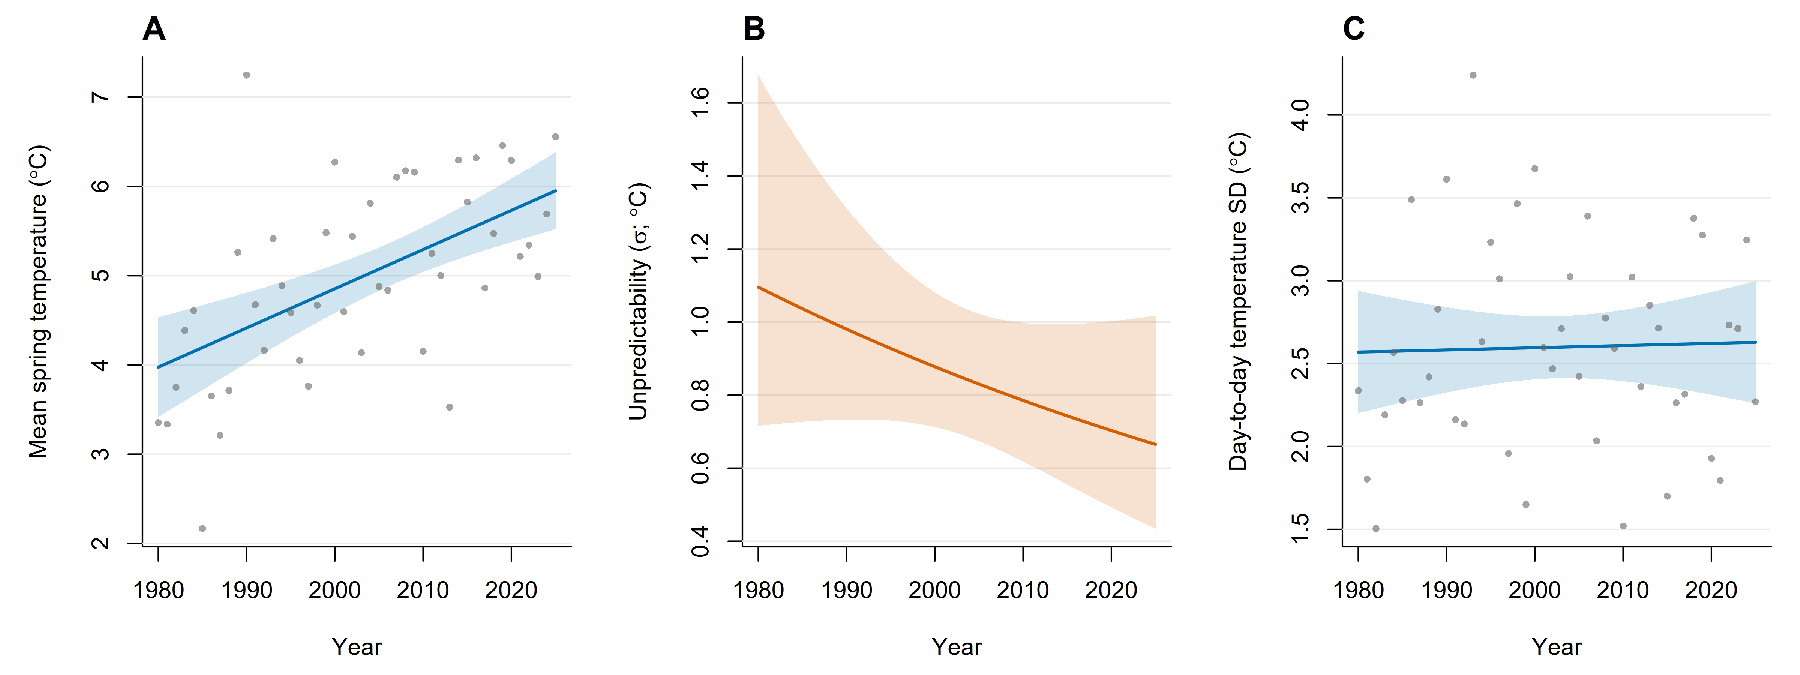
\includegraphics[width=.95\linewidth]{Fig2_temperature_location_scale_time.pdf}
\caption{Complete environmental predictions: (A) annual mean temperature, (B) residual interannual SD and (C) within-window daily SD. Points in A and C are observed annual summaries. Within-window daily SD in panel C is the sample standard deviation of the 43 daily mean temperatures within each season; it describes daily variation inside a season, separately from residual interannual variability in panel B. Lines and bands show fitted estimates and pointwise 95\% CIs; these environmental models contain no random effects.}
\label{sup-full-Fig2_temperature_location_scale_time}
\end{figure}

\begin{figure}[p]
\centering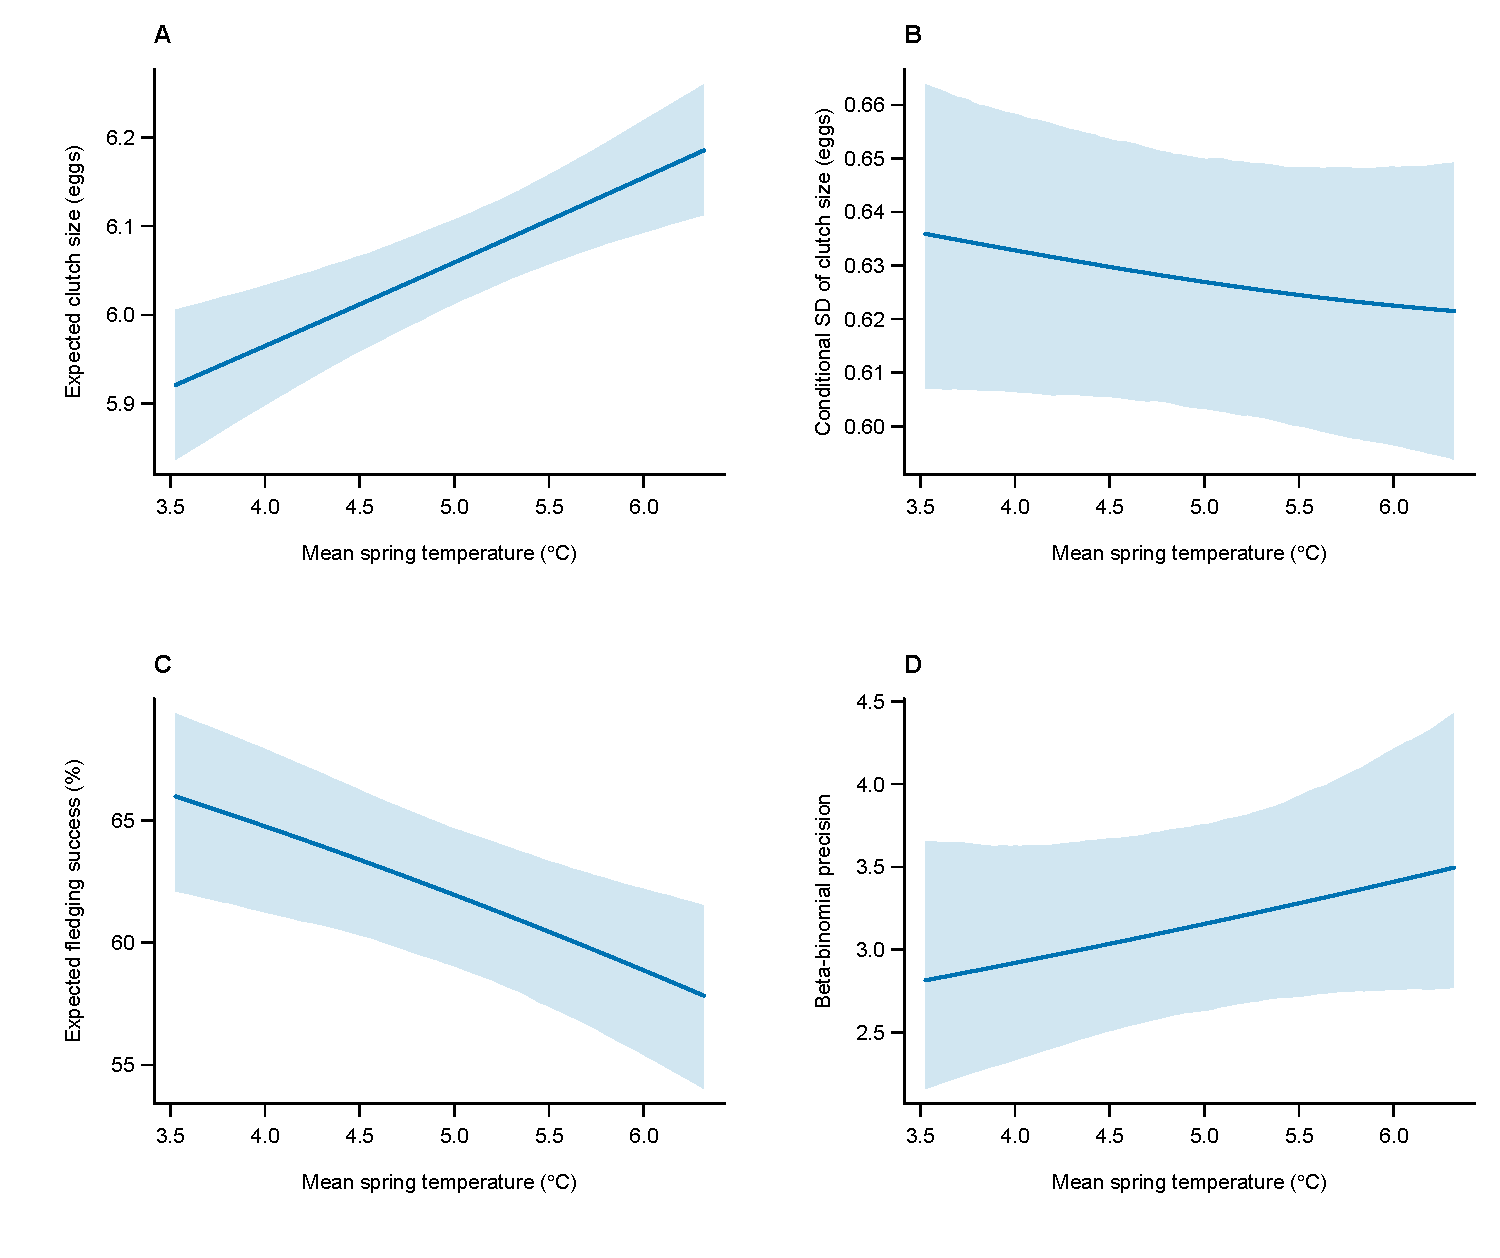
\includegraphics[width=.95\linewidth]{Fig_temperature_full_20261119.pdf}
\caption{Complete temperature predictions: (A) clutch mean, (B) clutch conditional SD, (C) full-mixture success and (D) component precision. Other reproductive predictors are held at reference values and random effects at zero. Bands and bars show pointwise 95\% CIs for the primary maximum-likelihood estimates.}
\label{sup-full-Fig3_COM_M1_temperature}
\end{figure}

\begin{figure}[p]
\centering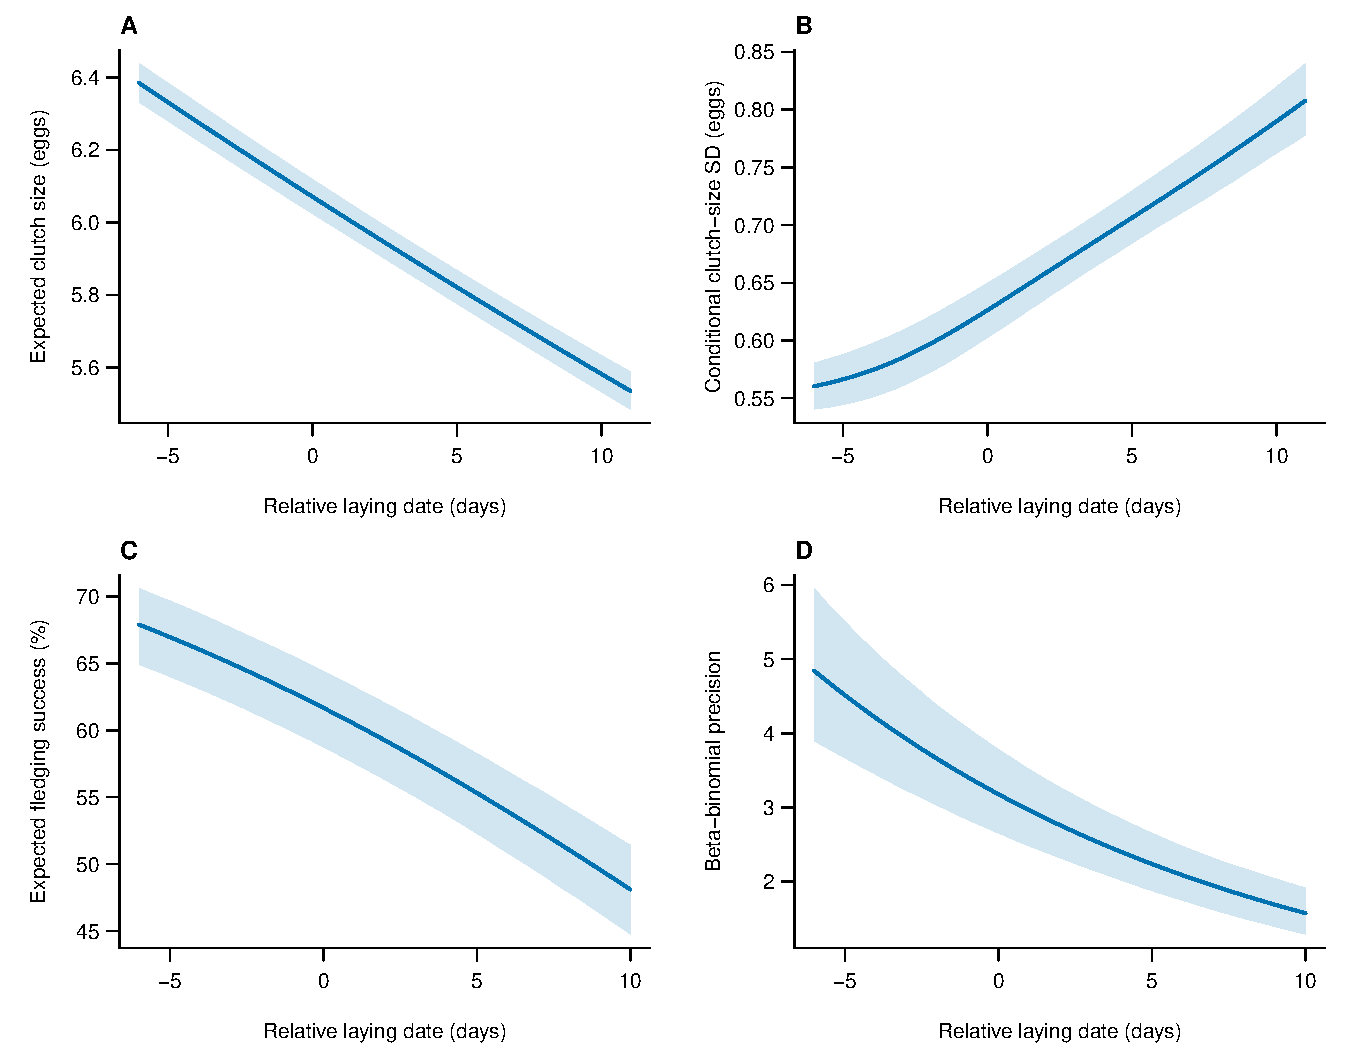
\includegraphics[width=.95\linewidth]{Fig_laying_date_20261119.pdf}
\caption{Complete date predictions: (A) clutch mean and (B) clutch conditional SD for yearlings; (C) full-mixture fledging success and (D) component precision for both age classes. The model has no age-by-date interactions. Other reproductive predictors are held at reference values and random effects at zero. Bands and bars show pointwise 95\% CIs for the primary maximum-likelihood estimates.}
\label{sup-full-Fig5_COM_M1_date}
\end{figure}

\begin{figure}[p]
\centering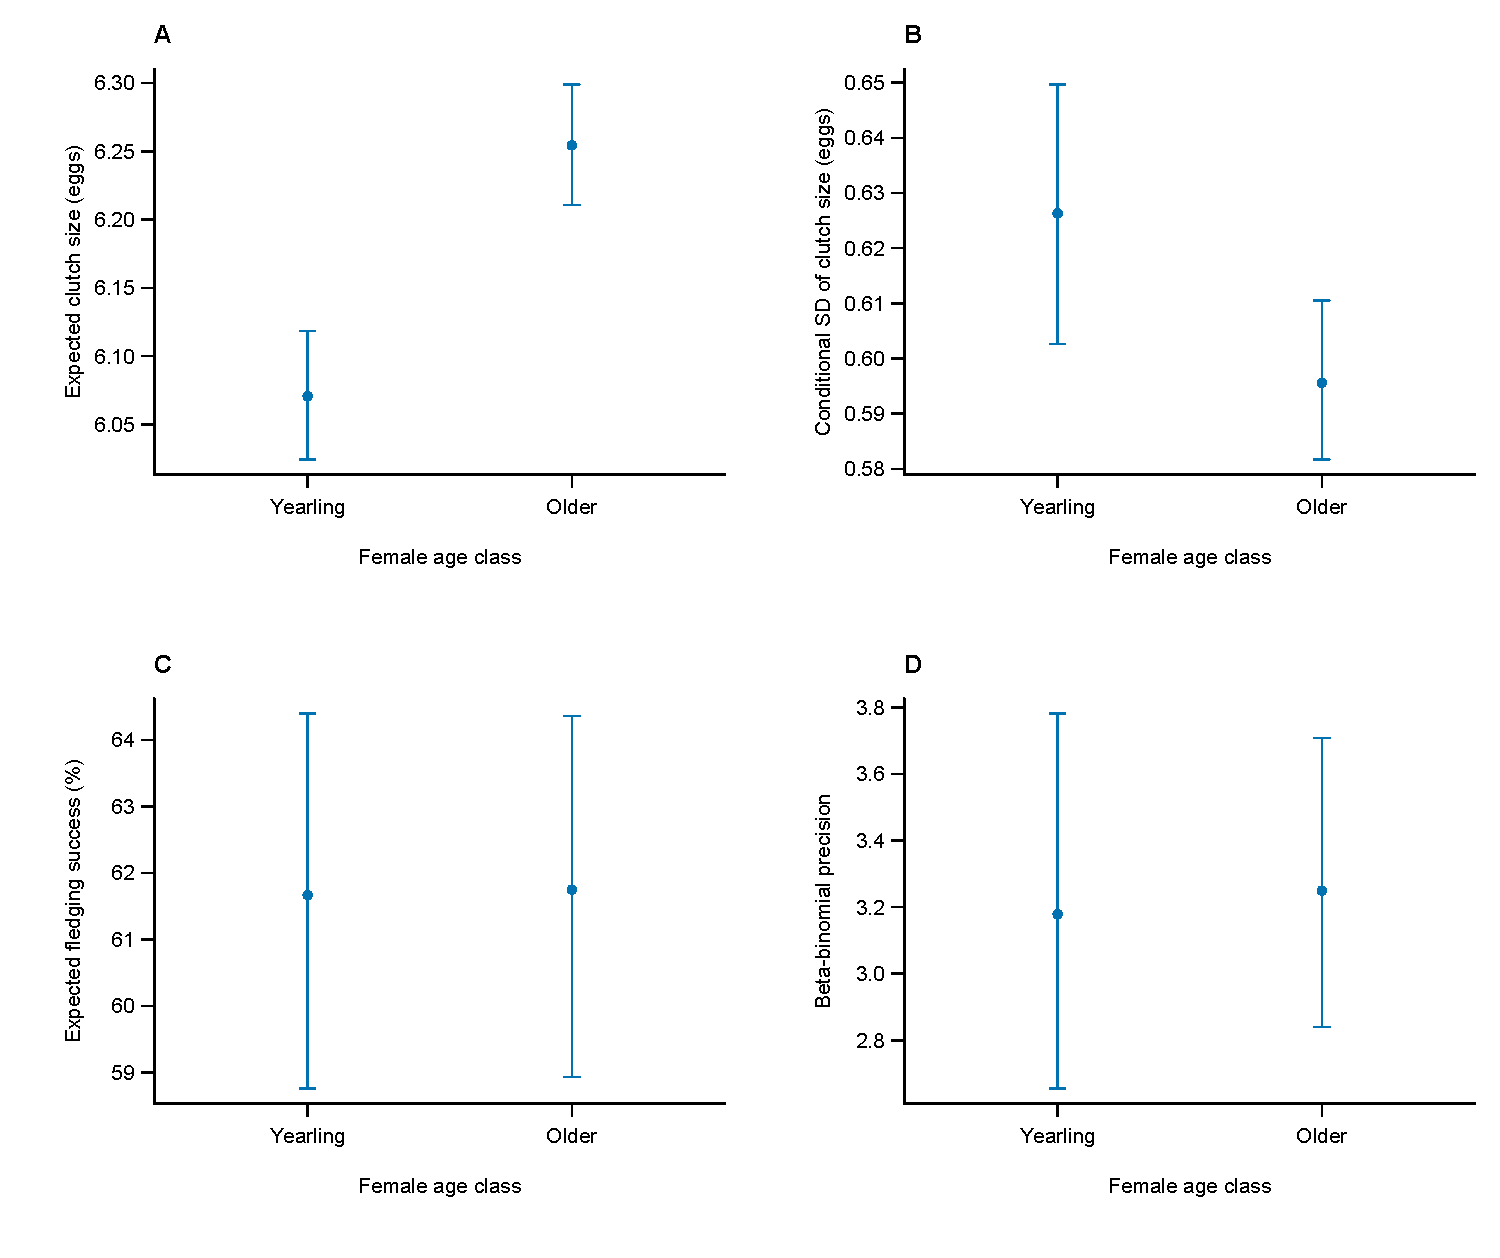
\includegraphics[width=.95\linewidth]{Fig_age_class_20261119.pdf}
\caption{Age-class predictions: (A) mean clutch size, (B) conditional clutch-size SD, (C) full-mixture expected egg-to-fledging success and (D) beta-binomial component precision. Yearlings are compared with older females; other predictors are at reference values and random effects are zero. Bars show pointwise 95\% CIs from the primary maximum-likelihood models.}
\label{sup-full-Fig7_female_age_location_scale}
\end{figure}

\clearpage
\begin{figure}[p]
\centering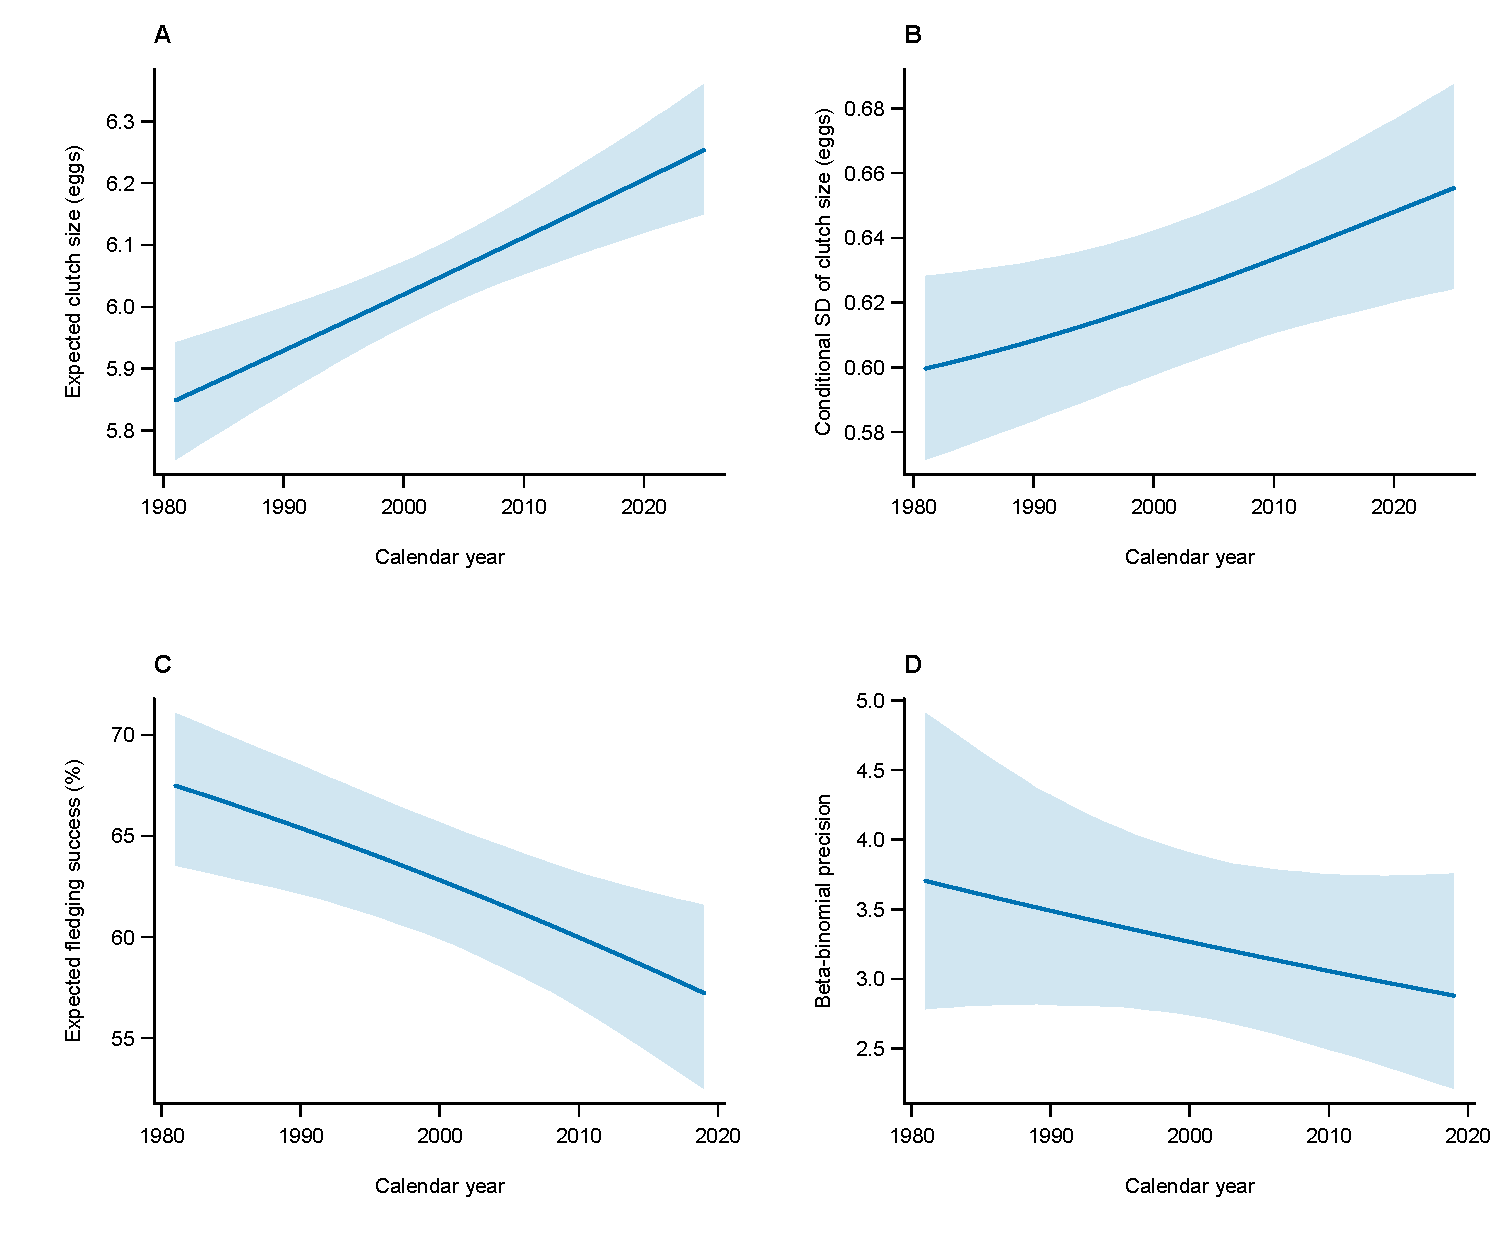
\includegraphics[width=.95\linewidth]{Fig_temporal_without_temperature_20261119.pdf}
\caption{Calendar-year predictions from models omitting temperature from location and scale while retaining age class, relative laying date and the original random effects: (A) expected clutch size, (B) conditional clutch-size SD, (C) full-mixture expected egg-to-fledging success and (D) beta-binomial component precision ($\phi$). Bands show pointwise 95\% CIs. Lower clutch-size SD indicates greater consistency; higher $\phi$ indicates greater consistency at a fixed component mean and clutch size.  }
\label{fig:reproductive-time}
\end{figure}

\begin{figure}[p]\centering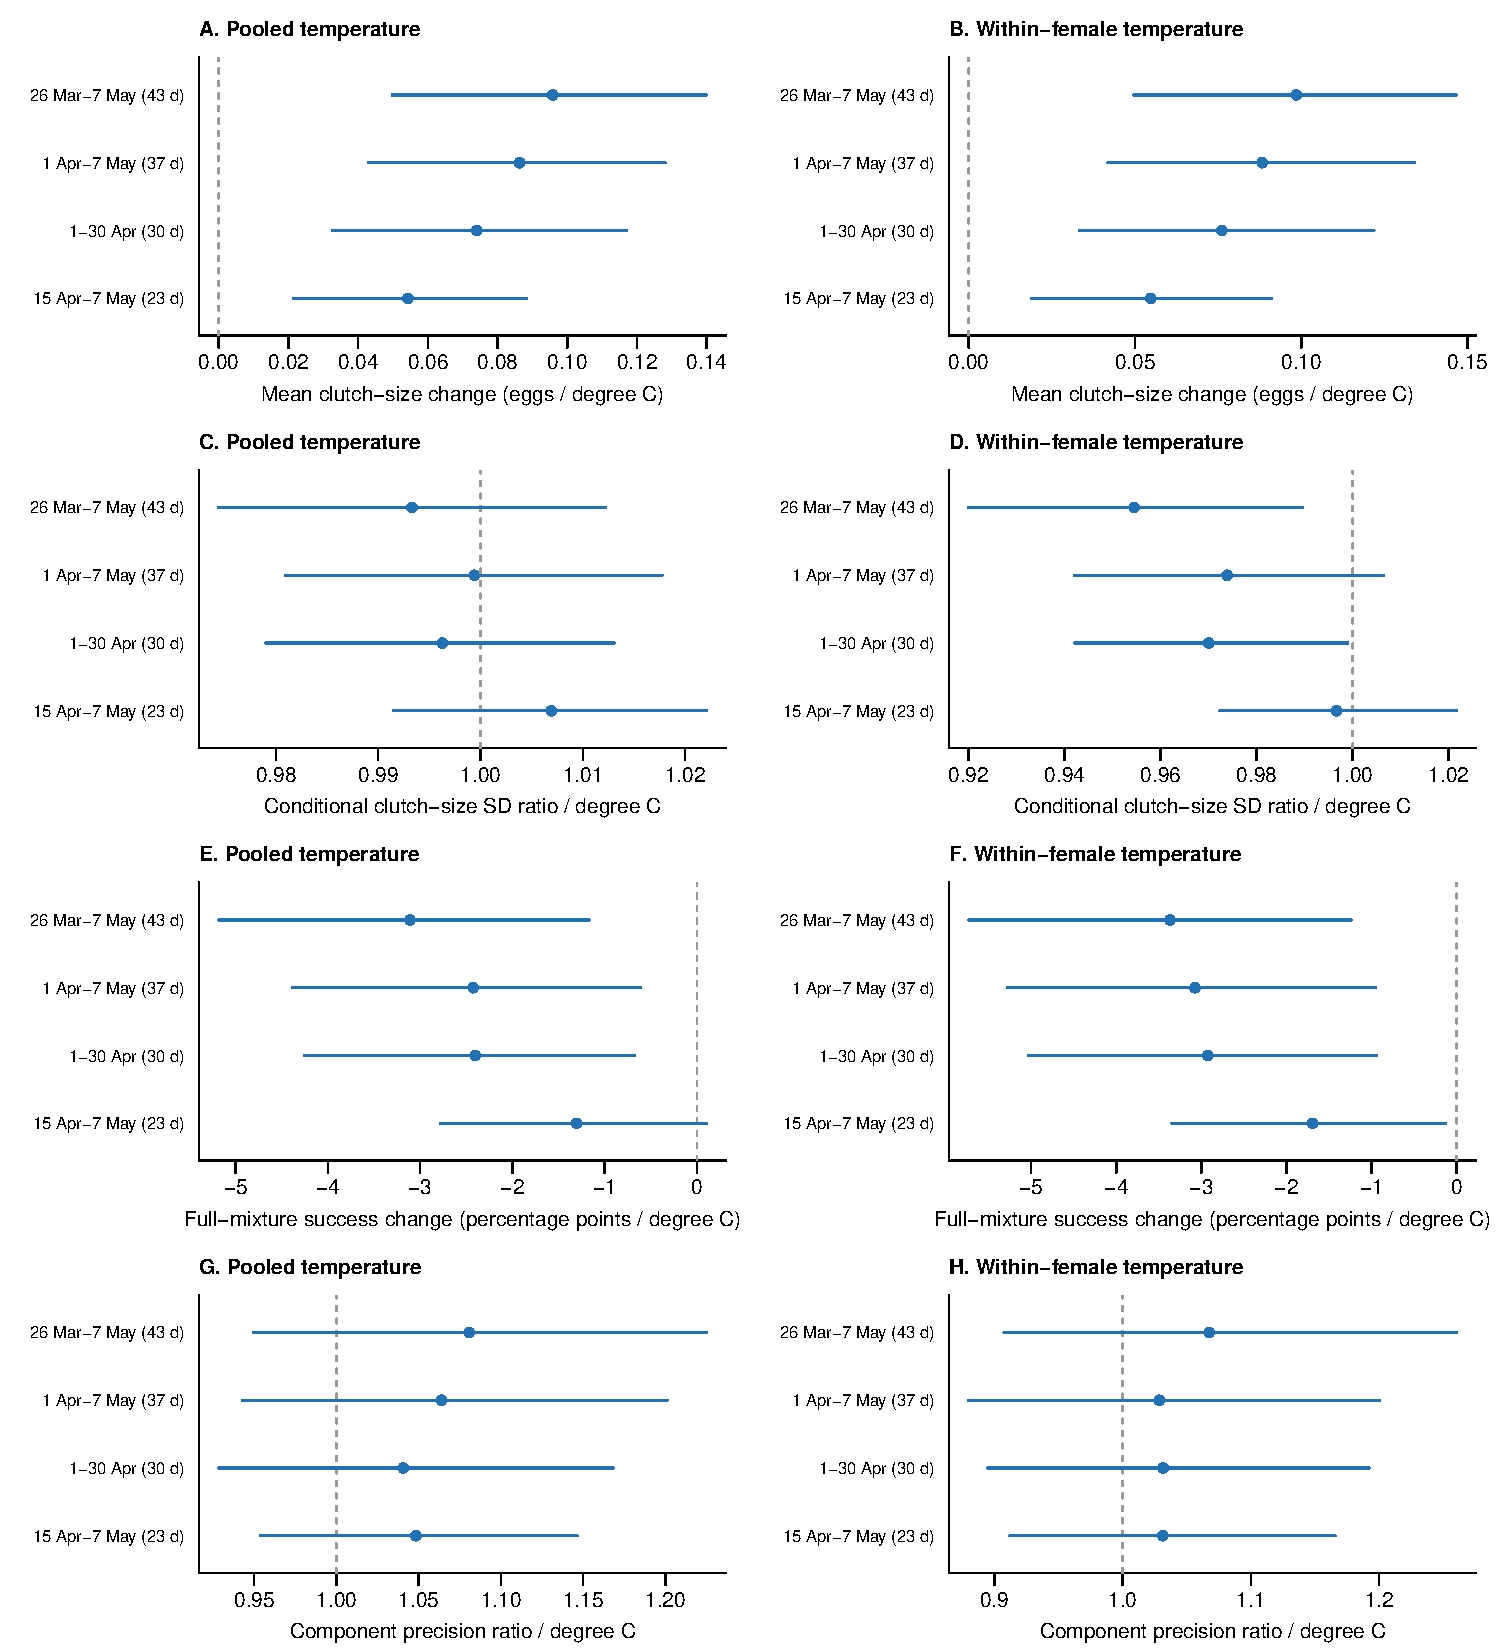
\includegraphics[width=.98\linewidth]{Fig_window_sensitivity_20261119.pdf}
\caption{Fixed-window sensitivity of pooled (left) and within-female (right) temperature associations. Points show contrasts per 1-degree increase from the centred reference and lines show 95\% coefficient-uncertainty intervals. Rows show mean clutch-size change, conditional clutch-size SD ratio, full-mixture fledging-success change and beta-binomial component-precision ratio. Every window uses identical trait-specific records. Vertical dashed lines indicate no mean change or a consistency ratio of one.}
\label{fig:window-sensitivity}\end{figure}

\clearpage
\bibliographystyle{plainnat}
\bibliography{refrences}
\end{document}
